\section{Experimental Results}
We provide our experimental results in this section. We compare the performance of
our ZO-PSVRG+  with 1) ZO-ProxSVRG (based on our improved analysis), 2) ZO-ProxSAGA-Coord \cite{gu2018faster} and 3) ZO-ProxSGD \cite{ghadimi2016accelerated} in experiments on two applications: black-box binary classification and adversarial attacks on black-box deep neural networks
(DNNs). We let ZO-ProxSGD denote RSPGF based on CoordSGE \eqref{gradestcoord} for gradient estimation. We also let ZO-ProxSVRG and ZO-ProxSVRG (RandSGE) denote respectively, ZO-PSVRG+  and ZO-PSVRG+ (RandSGE) with $\mathcal{B} = n$. The learning rates are tuned in the experiments for competitive algorithms according to their convergence guarantees in Table \ref{table-compare}, and the results shown in this section are based on the best learning rate we obtained for each algorithm. We set stepsize $\eta$ and smoothing parameter $\mu$ for ZO-PSVRG+ and ZO-PSVRG+ (RandSGE) according to the convergence guarantee we derived in lemmas and theorems.
\subsection{Black-Box Binary Classification}
In the first set of our experiments, we investigate logistic regression loss function with $L_1$ and $L_2$ regularization for training the black-box binary classification problem. The problem can be described as the optimization problem \eqref{problem} with $f_i(x) = \log(1+e^{-y_iz^T_i{x}})$, $h(x) = \lambda_1\|{x}\|_1 + \frac{\lambda_2}{2}\|{x}\|^2$, where $z_i\in\R^d$ and $y_i$ is the corresponding label for each $i$. The $L_1$ and $L_2$ regularization weights $\lambda_1$ and $\lambda_2$ are set respectively to $10^{-4}$ and $10^{-6}$, in all the experiments. We also set $\mathcal{B} = \lfloor{\frac{n}{5}}\rfloor$ for ZO-PSVRG+. We run our experiments on datasets from LIBSVM website{\footnote{https://www.csie.ntu.edu.tw/~cjlin/libsvmtools/datasets/binary.html}}, as listed in Table \ref{metadata}. The epoch size  is chosen as $m = 30$ in all of our experiments and the minibatch size  $b$ is fixed to $50$. 
 
\begin{table}[htbp]
\begin{center}
\caption{Summary of training datasets.}
\begin{tabular}{ c|c|c } 
 \hline
 Datasets &  Data & Features \\ 
 \hline
  ijcnn & 49990 & 22 \\
  a9a & 32561 & 123 \\ 
 w8a & 64,700  & 300 \\ 
 mnist & 60000 & 784 \\
%  \hline
% SUSY & 5,000,000 & 18 &  88,938,127 \\
 %epsilon &  400,000 & 2,000 &  800,000,000 \\
 %kdd12 & 119,705,032 & 54,686,452 & 0 \\
 \hline
\end{tabular}
\label{metadata}
\end{center}
\end{table}

\begin{figure*}[htbp]\vspace{-5mm}
\subfloat{
\centering
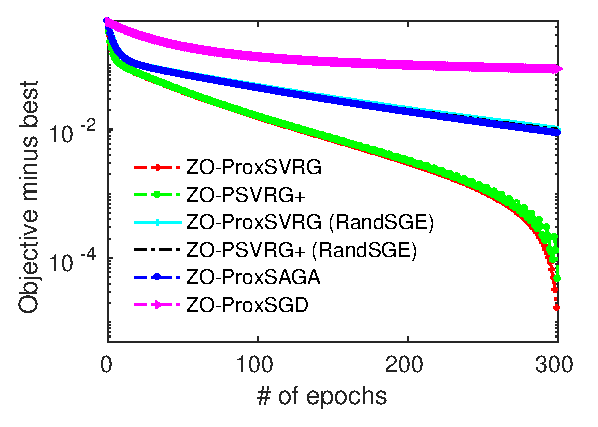
\includegraphics[width=0.23\linewidth]{Figures/binary/ijcnn1b50k1.eps}}%
\addtocounter{subfigure}{-4}
\subfloat{
\centering
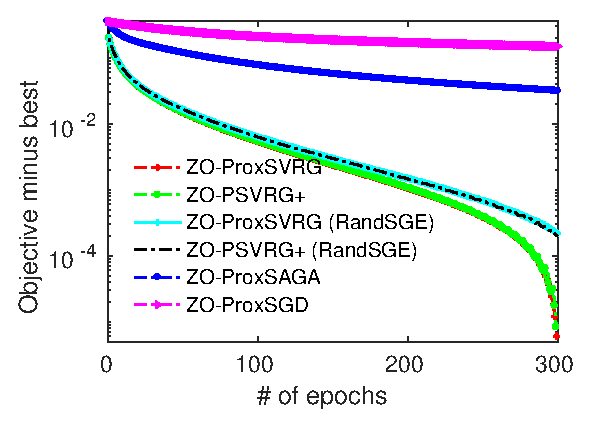
\includegraphics[width=0.23\linewidth]{Figures/binary/adultb50k1.eps}}%
\subfloat{
\centering
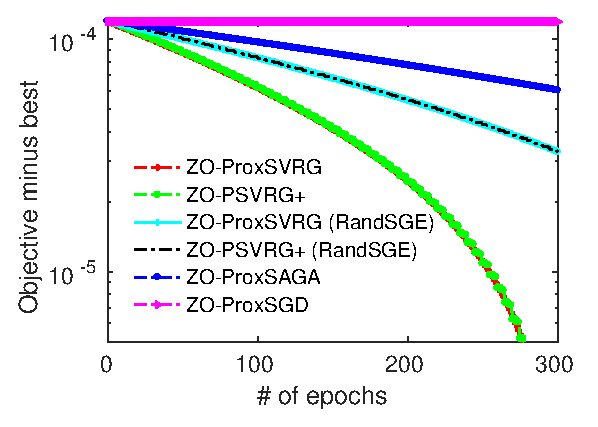
\includegraphics[width=0.23\linewidth]{Figures/binary/w8ab50k1.eps}}%
\subfloat{
\centering
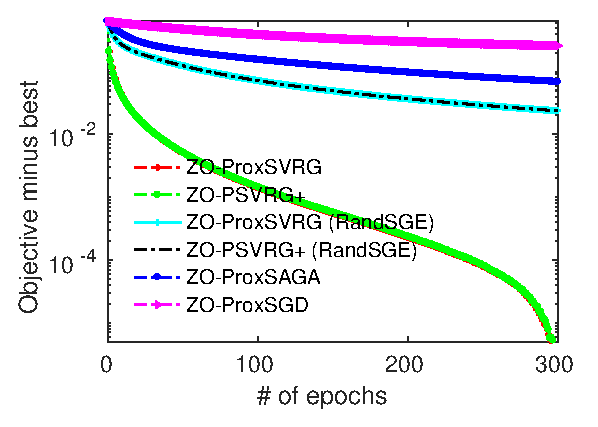
\includegraphics[width=0.23\linewidth]{Figures/binary/mnistb50k1.eps}}\\
\subfloat[ijcnn]{
\centering
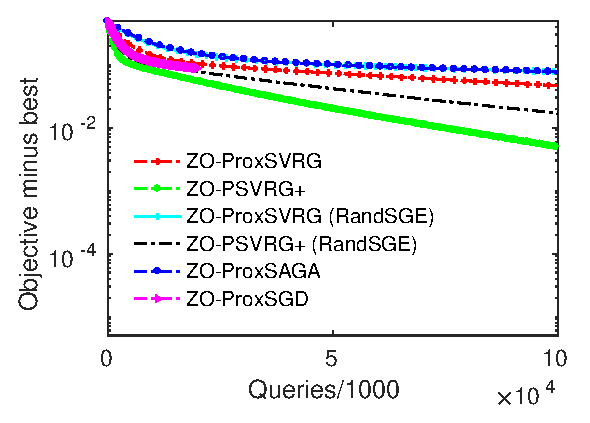
\includegraphics[width=0.23\linewidth]{Figures/binary/ijcnn1b50k2.eps}}%
\subfloat[comparison on covtype]{
\centering
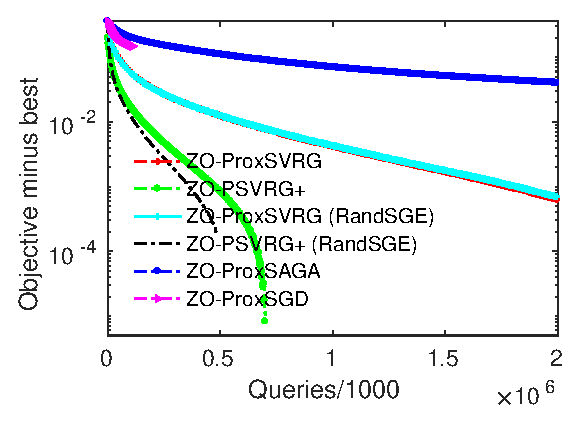
\includegraphics[width=0.23\linewidth]{Figures/binary/adultb50k2.eps}}%
\subfloat[w8a]{
\centering
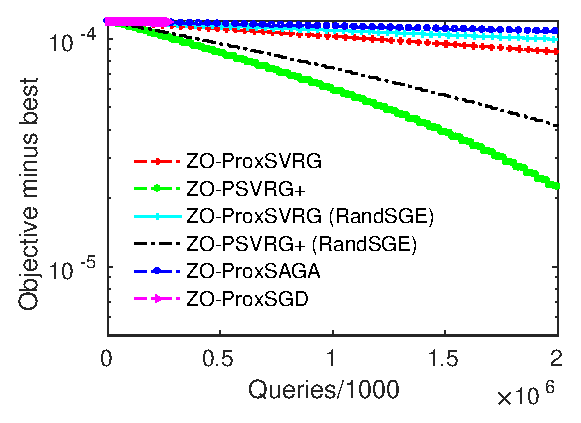
\includegraphics[width=0.23\linewidth]{Figures/binary/w8ab50k2.eps}}%
\subfloat[mnist]{
\centering
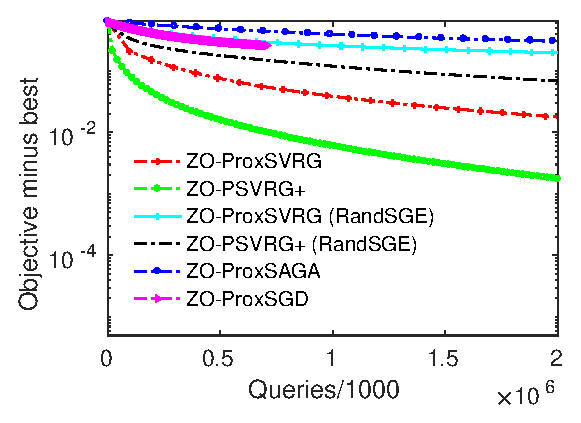
\includegraphics[width=0.23\linewidth]{Figures/binary/mnistb50k2.eps}}%
\setlength{\abovecaptionskip}{2pt}
\caption{Comparison of different zeroth-order algorithms for logistic regression loss residual $f(x) - f(x^*)$ versus the number of epochs (top) and ZO queries (bottom)}
\label{binary-fig}
\end{figure*}
In Figure \ref{binary-fig} (top), we show the training loss versus the number of epochs (i.e., iterations divided by the
epoch length $m = 30$). Note that ZO-PSVRG+ is evaluated using mix gradient CoordSGE \eqref{gradestcoord} and mix gradient RandSGE \eqref{gradestrand}.
Results in Figure \ref{binary-fig} (bottom) compare the performance of ZO-PSVRG+ with the variants of ZO variance reduced stochastic gradient descent described earlier in this section against the number of function queries. In these figures, we notice  a relatively faster convergence rate for ZO-PSVRG+ than the counterpart ZO-PSVRG+ (RandSGE). Note that ZO-ProxSVRG based on
our improved analysis have faster
convergence rate than ZO-ProxSAGA and also ZO-ProxSGD. On the other hand, the use of $\mathcal{B} = \lfloor{\frac{n}{5}}\rfloor$ in ZO-PSVRG+ significantly
improves ZO-ProxSVRG with respect to the number of ZO-queries (see Table \ref{table-compare}), leading to a non-dominant factor $O(I_{\{\mathcal{B} < n\}}/\mathcal{B})$ in the convergence rate of ZO-PSVRG+. Particularly ZO-PSVRG+ exhibits better performance in terms of number of function queries than ZO-ProxSAGA using CoordSGE.  The degradation in the convergence of ZO-ProxSAGA  is due to the requisite for small stepsizes $O(\frac{1}{d})$. Similarly, the large number of function queries to construct
coordinate-wise gradient estimates increases significantly the number of SZO queries for ZO-ProxSVRG. On the other hand, ZO-ProxSGD consumes an extremely large number of iterations while exhibiting marginal convergence compared with variance reduced algorithms. Thus, ZO-PSVRG+ obtains the best tradeoffs between the iteration and the function query complexity.





\subsection{Adversarial Attacks on Black-Box DNNs}
Adversarial 
examples in image classification are related to designing unperceptive perturbations such that they lead to misclassifying the target model by adding to the natural images. In the framework of zeroth-order attacks \cite{chen2017zoo,liu2018zeroth}, the model parameters are hidden and obtaining its gradient is not feasible, while only
the model evaluations are available. We can then consider the task of producing a universal adversarial
example with respect to $n$ natural images as an ZO optimization problem of the form \eqref{problem}.
More precisely, we apply the zeroth-order algorithms to obtain a global adversarial perturbation $x\in\R^d$ that could mislead the classifier on samples $\{a_i \in \R^d, y_i\in\mathbb{N} \}_{i=1}^n$. This problem can be specified as the following elastic-net attacks to black-box DNNs problem:
\begin{align}
\min_{x\in\R^d} \frac{1}{n} \sum_{i=1}^n& \max\{F_{y_i}(a_i^{adv}) - \max_{j\neq y_i}F_j(a_i^{adv}),0\}\notag\\
& + c\norm{a_i^{adv} - a_i}^2 + \lambda_1 \norm{x}_{1} + \lambda_2 \norm{x}^{2}\label{mnist-attack-loss}
\end{align}
where $a_i^{adv} = 0.5\tanh(\tanh^{-1}(2a_i)+x)$ and $\lambda_1$ and $\lambda_2$ are nonnegative parameters to obtain consistency between attack success rate, distortion and sparsity. Here $F(a) = \left[F_1(a),\ldots,F_K(a)\right]\in [0, 1]^K$ describes a trained DNN{\footnote{https://github.com/carlini/nn$\underline{~~}$robust$\underline{~~}$attacks}} for the MNIST handwritten digit classification, where $F_i(a)$ returns the prediction score of $i$-th class. The parameter $c$ in \eqref{mnist-attack-loss} compensates the rate of adversarial success and the distortion of adversarial examples. In our experiment, we set the regularization parameter  $c = 0.2$ and $\lambda_1 = \lambda_2  = 10^{-5}$.
\begin{figure}[htbp]
\subfloat[Loss vs iterations: $n = 10$]{
\centering
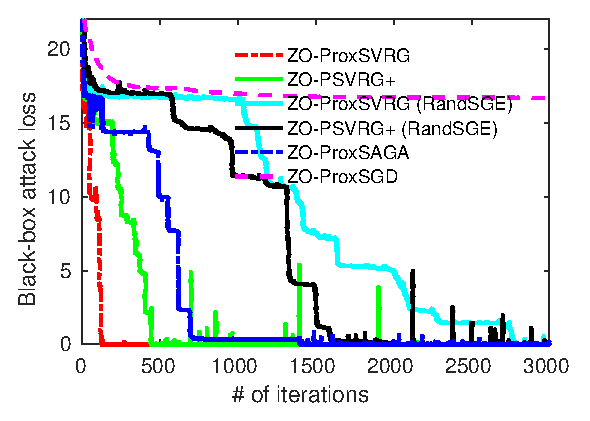
\includegraphics[width=0.44\linewidth]{Figures/attack/figiter.eps}}%
\subfloat[Loss vs queries: $n = 10$]{
\centering
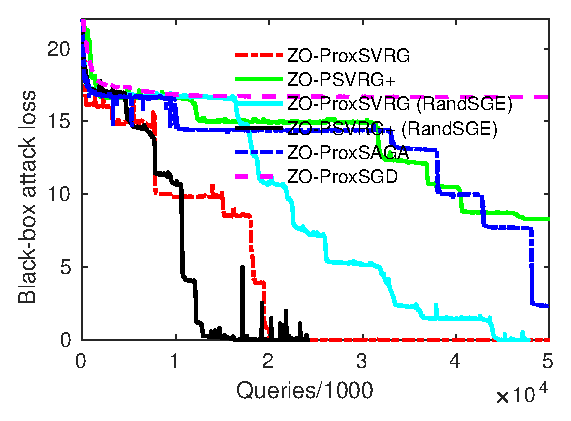
\includegraphics[width=0.44\linewidth]{Figures/attack/figquery.eps}}%
\setlength{\abovecaptionskip}{2pt}
\caption{Comparison of different zeroth-order algorithms for generating black-box adversarial examples from a black-box DNN}
\label{attack-fig}
\end{figure}
We perform two experiments by choosing $n = 10$ and $n=100$ images from the same class, and set the minibatch sizes, respectively $b=5$ and $b = 30$. We select the batch size $\mathcal{B} = \lfloor{\frac{n}{2}}\rfloor$ for ZO-PSVRG+.
Figure \ref{attack-fig} shows
the performance of different ZO algorithms considered in this paper. Our two algorithms ZO-PSVRG+ (RandSGE) and ZO-ProxSVRG (under our improved analysis) show better performance
both in convergence rate (iteration complexity) and function query complexity than ZO-ProxSGD
and ZO-ProxSAGA. The performance of ZO-PSVRG+ (CoordSGE) algorithm degrades due to large number of function queries for CoordSGE and the variance inherited by $\mathcal{B} \neq n$. 
ZO-PSVRG+ (RandSGE) shows faster convergence in the initial optimization stage, and more importantly, has much lower function query complexity, which is largely
due to efficient ZO queries for computing mix gradient \eqref{zo-grad-fo-rand} and  the $O(\frac{1}{\sqrt{d}})$-level stepsize required by ZO-PSVRG+ (RandSGE). ZO-ProxSAGA and ZO-PSVRG+ (CoordSGE) exhibit relatively similar convergence behaviors. Furthermore, the convergence performance of ZO-ProxSGD is poor compared to other algorithms due to not using variance reduced techniques. 
\iffalse
\ref{fig:FSVRG_compare} shows the convergence of the objective function with respect to CPU time and the number of iterations. 
\begin{figure}[htbp]
\subfloat[a]{
\centering
\includegraphics[width=0.44\linewidth]{Figures/figure_logistic_rcv_update_32_time.eps}}%
\hfill
\subfloat[b]{
\centering
\includegraphics[width=0.44\linewidth]{Figures/figure_logistic_rcv_update_32_iteration.eps}}%
\caption{Figure(a) is convergence of objective value vs. time; Figure(b) is comparison of the objective function vs. iteration for different algorithms.}
\label{fig:FSVRG_compare}
\end{figure}
\fi

